%!TEX TS-program = pdflatexmk

% Copyright (c) 2018 - 2022, Martin Scheidt (ISC license)
% Permission to use, copy, modify, and/or distribute this file for any purpose with or without fee is hereby granted, provided that the above copyright notice and this permission notice appear in all copies.

\documentclass[border=2]{standalone}

\usepackage[dev]{tikz-trackschematic}

\begin{document}
  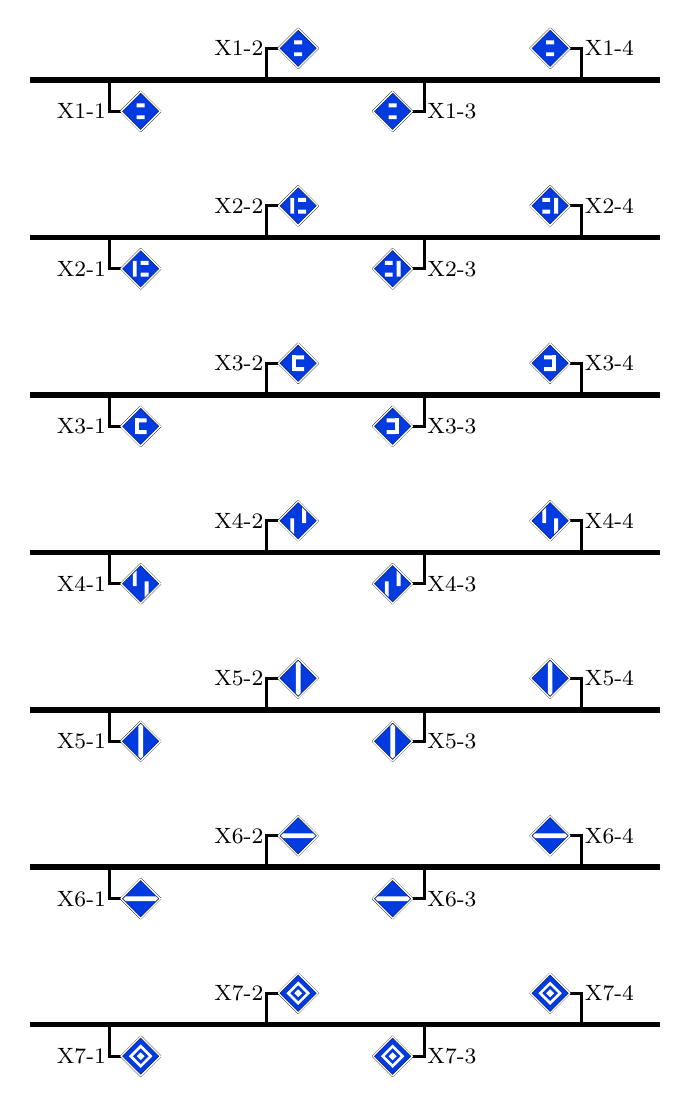
\begin{tikzpicture}
  
    \foreach \i in {1,2,...,7}{% base coordinate
      \coordinate (A\i) at ($(0,0) + 2*(0,-\i)$);% base coordinate
      \coordinate (B\i) at ($(8,0) + 2*(0,-\i)$);% base coordinate
      %
      \maintrack (A\i) --   (B\i); % draw main tracks on base coordinate
      %
      % coordinates for testing symbols
      \coordinate (X\i-1) at ($(1,0) + 2*(0,-\i)$);
      \coordinate (X\i-2) at ($(3,0) + 2*(0,-\i)$);
      \coordinate (X\i-3) at ($(5,0) + 2*(0,-\i)$);
      \coordinate (X\i-4) at ($(7,0) + 2*(0,-\i)$);
    }

    \distantpoweroff[forward ] at (X1-1) label (X1-1);
    \distantpoweroff[forward ,position=left] at (X1-2) label (X1-2);
    \distantpoweroff[backward,position=left] at (X1-3) label (X1-3);
    \distantpoweroff[backward] at (X1-4) label (X1-4);

    \poweroff[forward ] at (X2-1) label (X2-1);
    \poweroff[forward ,position=left] at (X2-2) label (X2-2);
    \poweroff[backward,position=left] at (X2-3) label (X2-3);
    \poweroff[backward] at (X2-4) label (X2-4);

    \poweron[forward ] at (X3-1) label (X3-1);
    \poweron[forward ,position=left] at (X3-2) label (X3-2);
    \poweron[backward,position=left] at (X3-3) label (X3-3);
    \poweron[backward] at (X3-4) label (X3-4);

    \distantpantographdown[forward ] at (X4-1) label (X4-1);
    \distantpantographdown[forward ,position=left] at (X4-2) label (X4-2);
    \distantpantographdown[backward,position=left] at (X4-3) label (X4-3);
    \distantpantographdown[backward] at (X4-4) label (X4-4);

    \pantographdown[forward ] at (X5-1) label (X5-1);
    \pantographdown[forward ,position=left] at (X5-2) label (X5-2);
    \pantographdown[backward,position=left] at (X5-3) label (X5-3);
    \pantographdown[backward] at (X5-4) label (X5-4);

    \pantographup[forward ] at (X6-1) label (X6-1);
    \pantographup[forward ,position=left] at (X6-2) label (X6-2);
    \pantographup[backward,position=left] at (X6-3) label (X6-3);
    \pantographup[backward] at (X6-4) label (X6-4);

    \wirelimit[forward ] at (X7-1) label (X7-1);
    \wirelimit[forward ,position=left] at (X7-2) label (X7-2);
    \wirelimit[backward,position=left] at (X7-3) label (X7-3);
    \wirelimit[backward] at (X7-4) label (X7-4);

  \end{tikzpicture}
\end{document}